\chapter{Variabilidad entre los datos de entrenamiento y testeo}
\label{variabilidad}
A pesar de todos las técnicas aplicadas en los capítulos anteriores, no ha sido posible para SVM igualar la performance de RF en varios de los tiles analizados. Dado que es esperable que SVM lineal sea incapaz de alcanzar la performance de RF por su limitación de generar superficies de decisión no lineales, en este capítulo nos concentraremos en entender qué está limitando a SVM-RBF. \\

Una hipótesis que fue sugerida en la sección \ref{analisis_distribuciones} es que el problema se encuentra en el hecho de que las distribuciones de probabilidad subyacentes a cada tile parecen ser significativamente distintas. En las distintas secciones de este capítulo se analizará esta hipótesis en detalle.

\section{Impacto de la variabilidad de datos en la elección de hiperparámetros }
\label{impacto}
Es importante resaltar que la performance de SVM-RBF es extremadamente sensible a la elección de hiperparámetros, como se pudo observar en la figura \ref{fig:optimisationsvmk}. Pequeñas variaciones de $C$ y $\gamma$ pueden ocasionar saltos significativos en el R-AUPRC obtenido. Por otro lado, una de las virtudes más reconocidas de RF es el hecho de que no requiere una optimización muy cuidadosa de hiperparámetros, siendo un método off-the-shelf \cite{offshelf}. \\

Es posible que los hirparámetros $C$ y $\gamma$ que se estimaron en capítulos anteriores realizando cross-validation sobre un único tile ($b278$) no produzcan buenos resultados al utilizarse para entrenar y testear SVM utilizando otros pares de tiles. Para aclarar esto, se condujo un experimento que responderá a la siguiente pregunta:

\begin{quotation}
Dado un par de tiles arbitrario $t_1$ y $t_2$. ¿Existe una combinación de hiperparámetros $C$ y $\gamma$ tal que SVM-RBF entrenado con $t_1$ tenga igual o mejor R-AUPRC en test que RF, testeando en $t_2$?
\end{quotation}

Se calculó el R-AUPRC en test para cada combinación de hiperparámetros de una grilla de valores de $\gamma$ y $C$, entrenando y testeando SVM-RBF en cada par de tiles. Los resultados se encuentran en las figuras \ref{fig:poder_predictivo} y \ref{fig:poder_predictivo_curvas}. A partir de estos datos, podemos observar lo siguiente:

\begin{itemize}
\item En primer lugar, observando las curvas de la figura \ref{fig:poder_predictivo_curvas}, podemos ver que la performance de RF ya no es marcadamente superior a la de SVM, debido a las mejoras que se introdujeron en los capítulos anteriores. Sin embargo, RF continúa teniendo mejor performance en varios de los pares testeados.
\item Una segunda observación que se desprende de las curvas de la figura \ref{fig:poder_predictivo_curvas} es que, en general, los hiperparámetros que se seleccionaron para SVM-RBF en capítulos anteriores ($C=10^4$ y $\gamma=10^{-4}$) son casi tan buenos como los hiperparámetros óptimos en cada par de tiles. Es decir, la elección de hiperparámetros que se venía utilizando generaliza de forma apropiada.
\item Podemos ver que la asignación de hiperparámetros que mejor funciona en un cierto par de tiles, a menudo funciona muy mal en otro. Por ejemplo, escoger $ 10^{-4} \leq \gamma \leq 10^{-2}$ y $ 10^5 \leq C \leq 10^{11}$ produce resultados óptimos en $b278 \mapsto b261$, en tanto que produce consistentemente los peores resultados cada vez que se entrena con $b234$. Esto sugiere que es complicado (o imposible) hallar una asignación de hiperparámetros que sea óptima para todo par de tiles. Dicho esto, se vuelve a remarcar que la asignación de parámetros que se venía utilizando ($C=10^4$ y $\gamma=10^{-4}$), si bien no es óptima en todos los tiles, es una de las pocas que se encuentra consistentemente entre las que mejor funcionan en distintos tiles.
\item Prestando atención a las celdas tachadas en la figura \ref{fig:poder_predictivo} y a las curvas de la figura \ref{fig:poder_predictivo_curvas}, se observa que SVM-RBF (incluso sobreajustando los hiperparámetros) no es capaz de empatar la performance de RF en cuatro de las combinaciones testeadas: $b234 \mapsto b360$, junto con todos los tiles entrenados en $b360$. El hecho de que el tile  $b360$ esté involucrado en todos estos pares puede estar relacionado al hecho de que $b360$ se encuentra espacialmente a mayor distancia de $b234$, $b261$ y $b278$ (ver figura \ref{fig:vvv_tiles}). Esto podría ocasionar que la distribución subyacente de $b360$ sea más diferente a la de los otras tres tiles, siendo más difícil que clasificadores entrenados en otros tiles generalicen bien.
\end{itemize}


\begin{figure}[h!]
\begin{tabular}{cccc}
  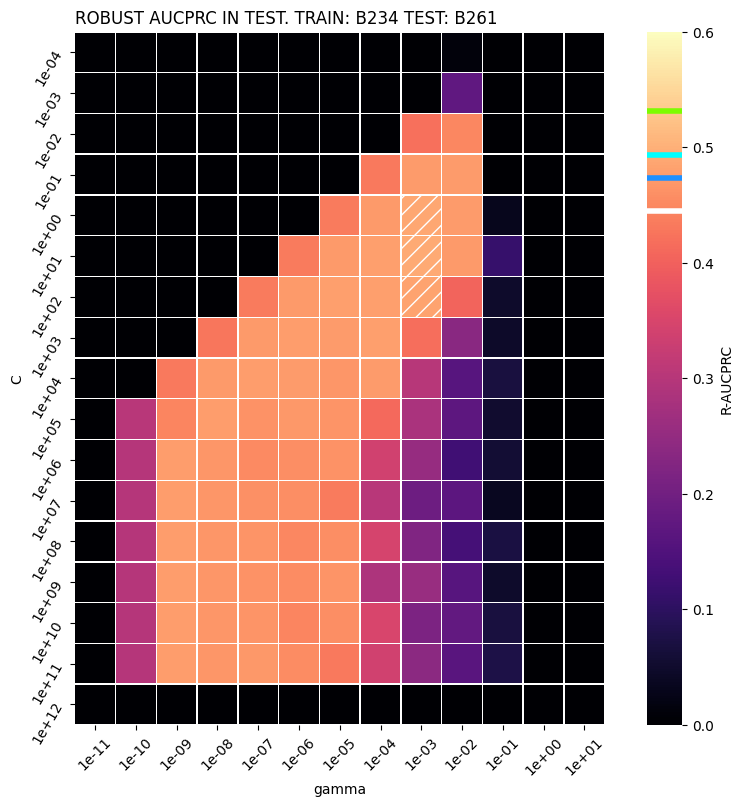
\includegraphics[width=0.25\textwidth]{Kap8/heatmap_train=b234_test=b261.png}  
  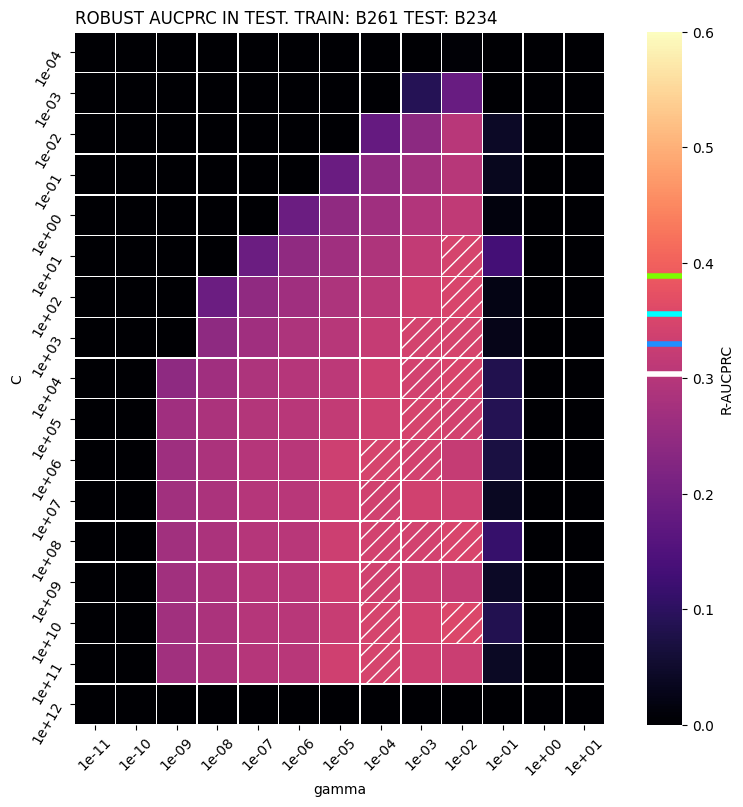
\includegraphics[width=0.25\textwidth]{Kap8/heatmap_train=b261_test=b234.png}
  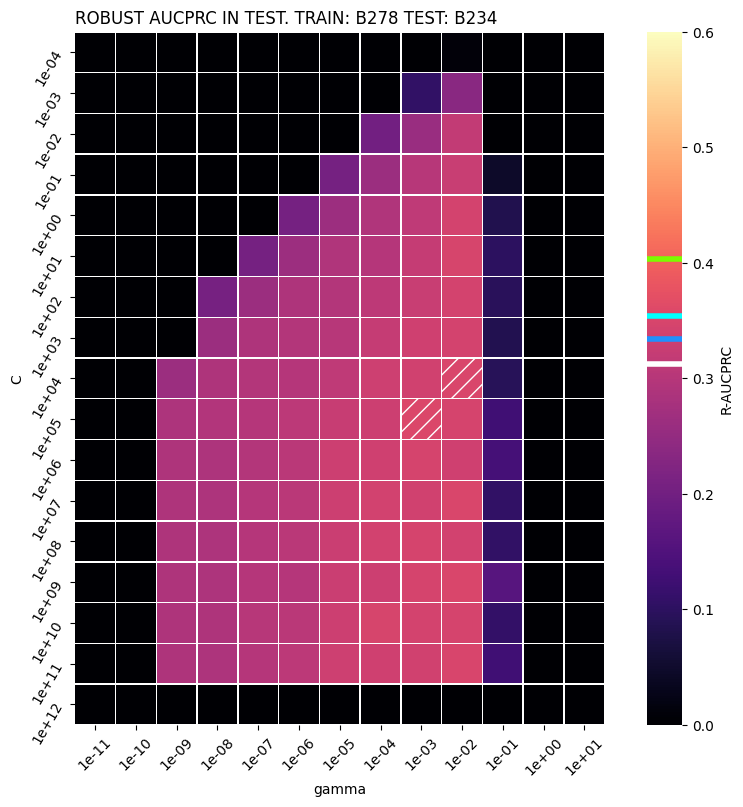
\includegraphics[width=0.25\textwidth]{Kap8/heatmap_train=b278_test=b234.png} 
   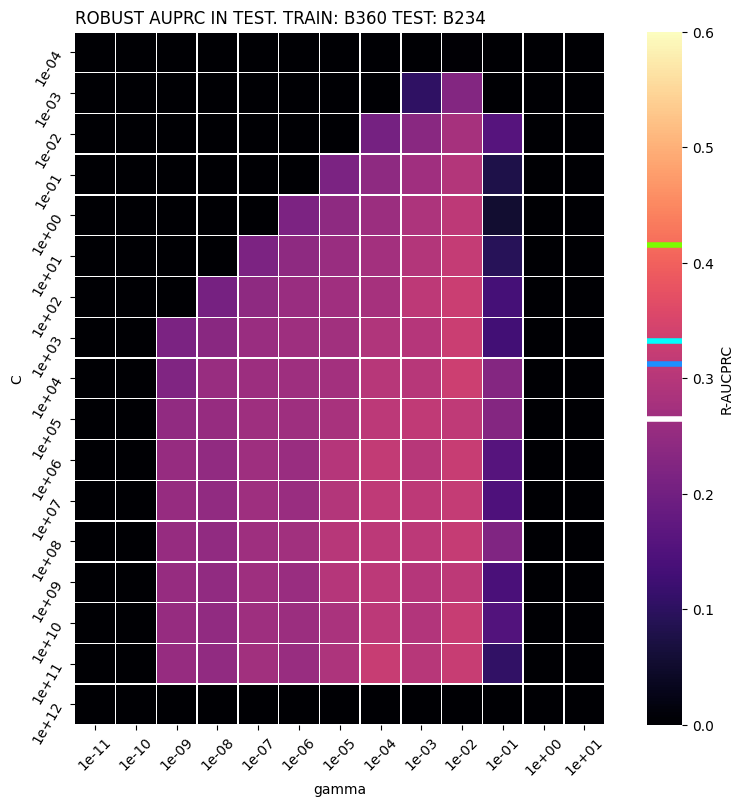
\includegraphics[width=0.25\textwidth]{Kap8/heatmap_train=b360_test=b234.png} \\

  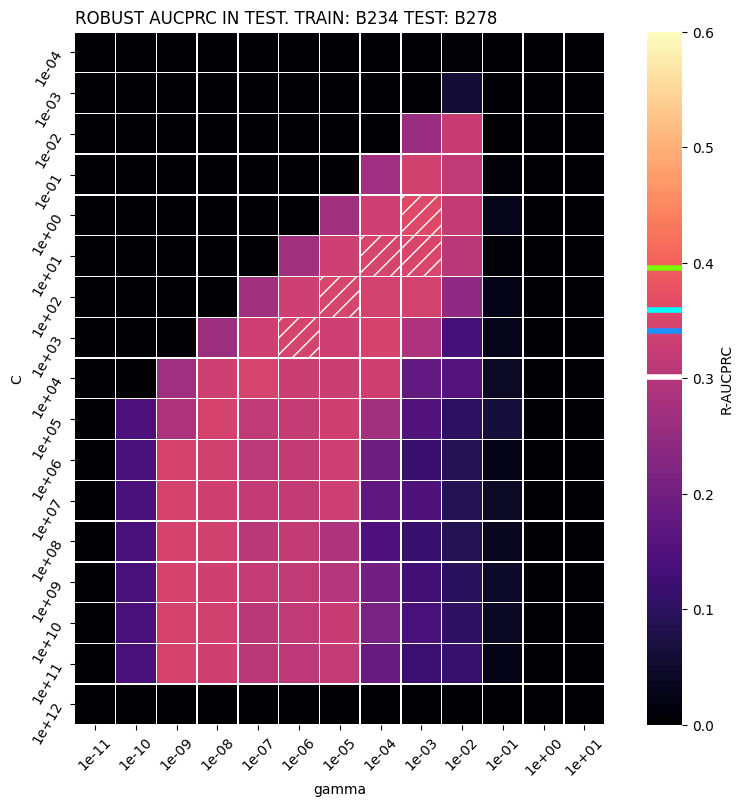
\includegraphics[width=0.25\textwidth]{Kap8/heatmap_train=b234_test=b278.png}  
  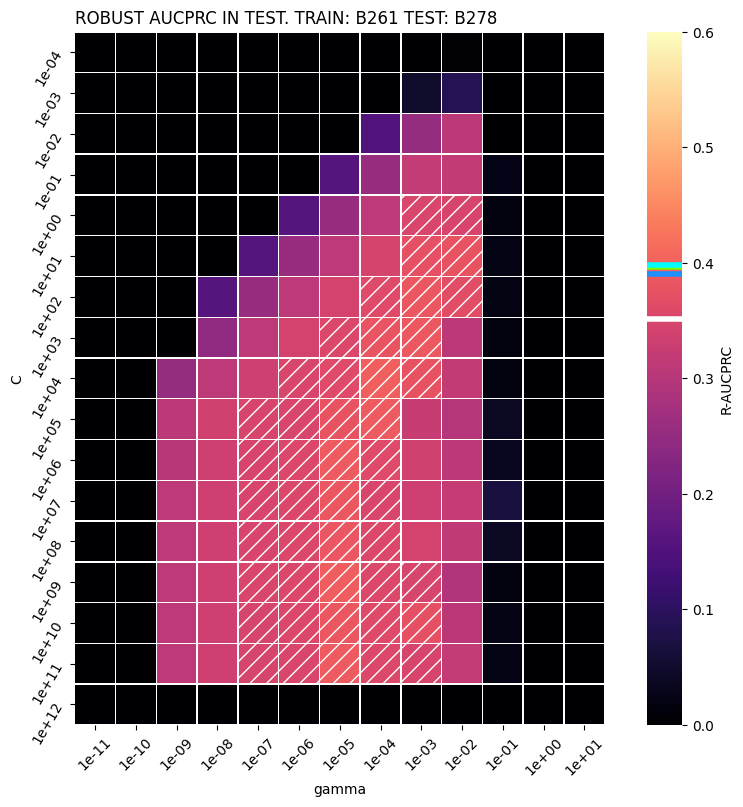
\includegraphics[width=0.25\textwidth]{Kap8/heatmap_train=b261_test=b278.png}
  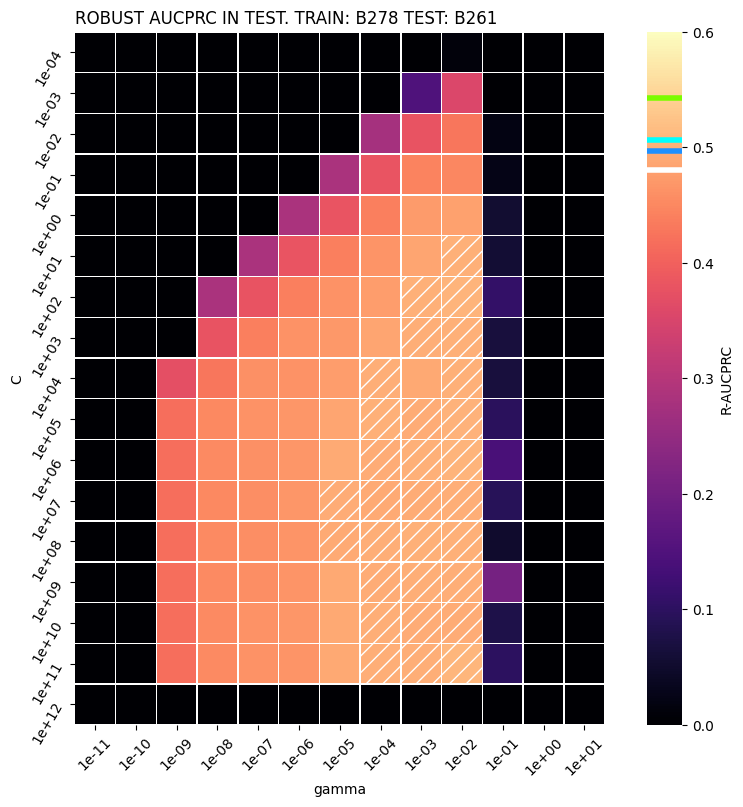
\includegraphics[width=0.25\textwidth]{Kap8/heatmap_train=b278_test=b261.png} 
   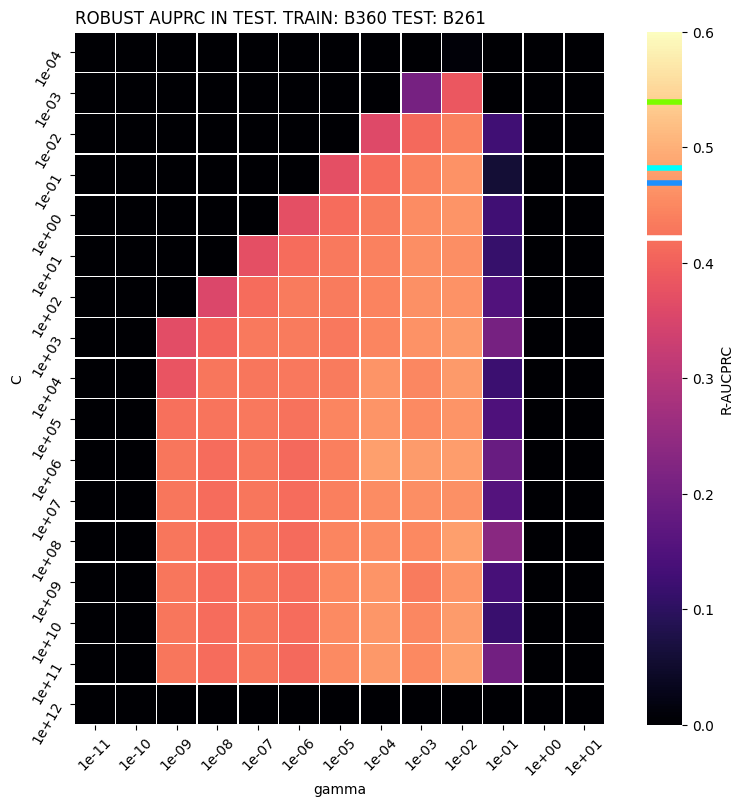
\includegraphics[width=0.25\textwidth]{Kap8/heatmap_train=b360_test=b261.png} \\
   
     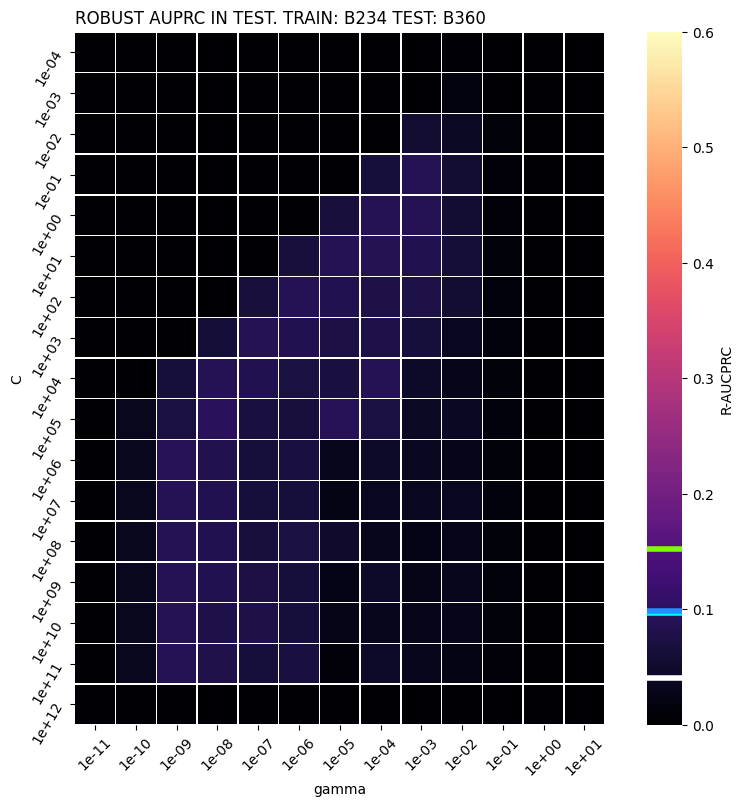
\includegraphics[width=0.25\textwidth]{Kap8/heatmap_train=b234_test=b360.png}  
  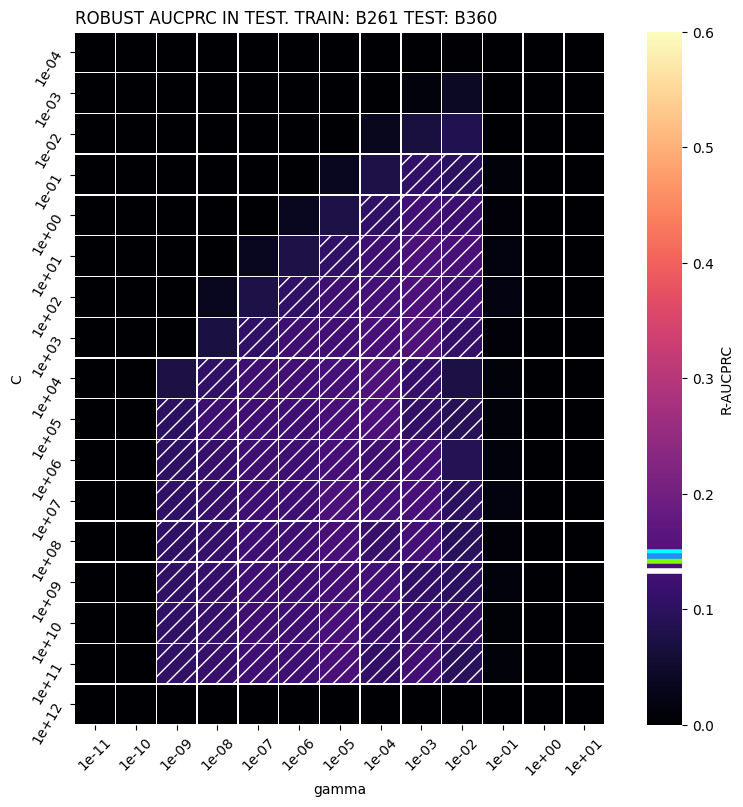
\includegraphics[width=0.25\textwidth]{Kap8/heatmap_train=b261_test=b360.png}
  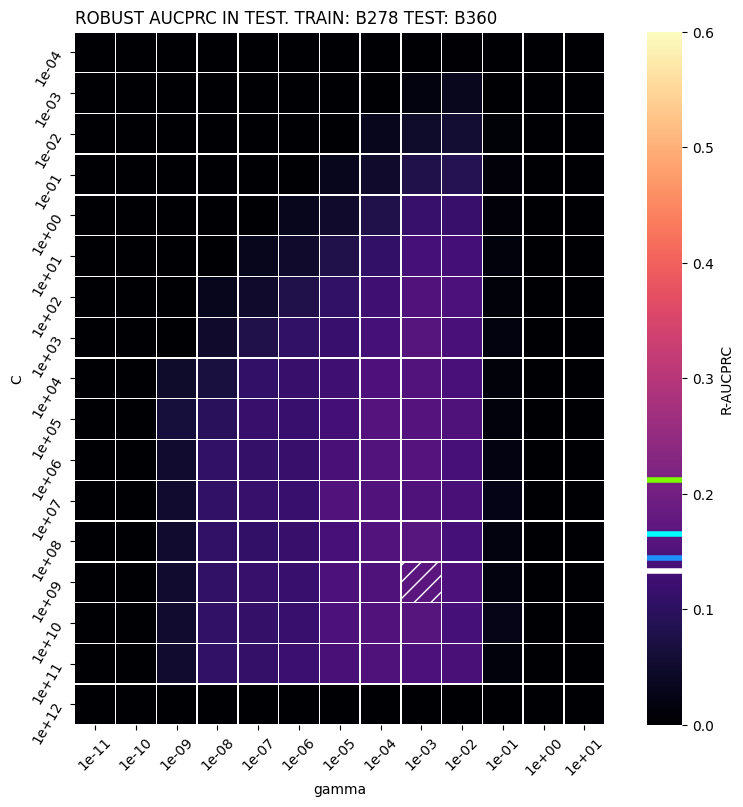
\includegraphics[width=0.25\textwidth]{Kap8/heatmap_train=b278_test=b360.png} 
   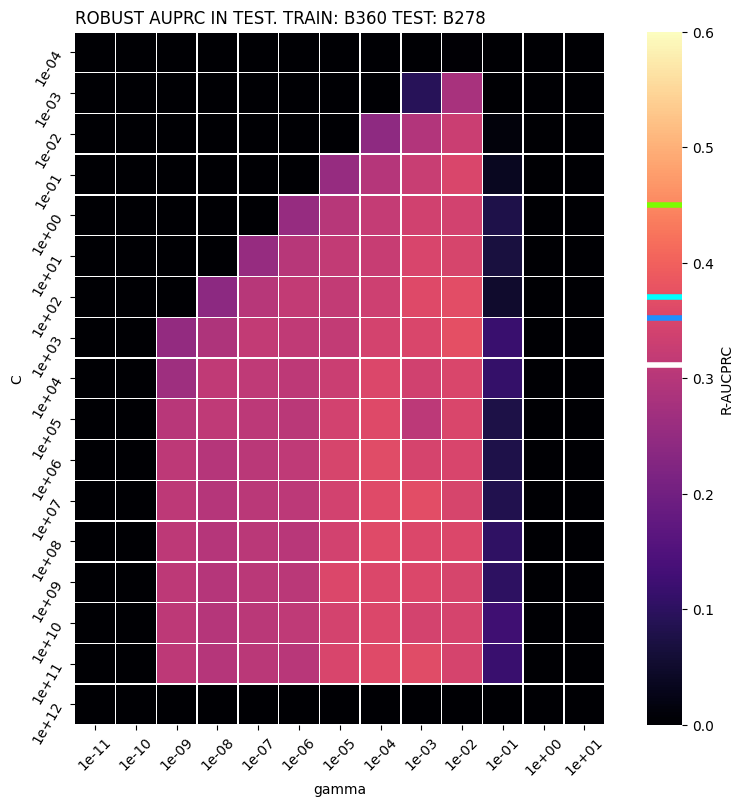
\includegraphics[width=0.25\textwidth]{Kap8/heatmap_train=b360_test=b278.png} \\

\end{tabular}
\caption{Cada grilla muestra el R-AUPRC en test obtenido utilizando SVM-RBF con distintos hiperparámetros en distintos pares de tiles. En la barra de color se marca, con líneas horizontales, el R-AUPRC de Random Forest (verde), el valor óptimo de SVM-RBF encontrado en esta grilla (celeste), junto con los mejores resultados obtenidos en el capítulo anterior para SVM-RBF (azul) y SVM-Lineal (blanco). Adicionalmente, se tacharon aquellas celdas individuales cuyo R-AUPRC está a menos de 0.5 del de RF. }
\label{fig:poder_predictivo}
\end{figure}

\begin{figure}[h!]
\begin{tabular}{cccc}
  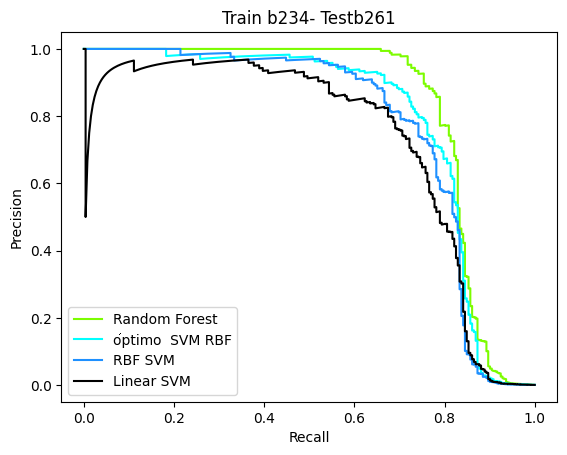
\includegraphics[width=0.25\textwidth]{Kap8/best-train=b234test=b261.png}  
  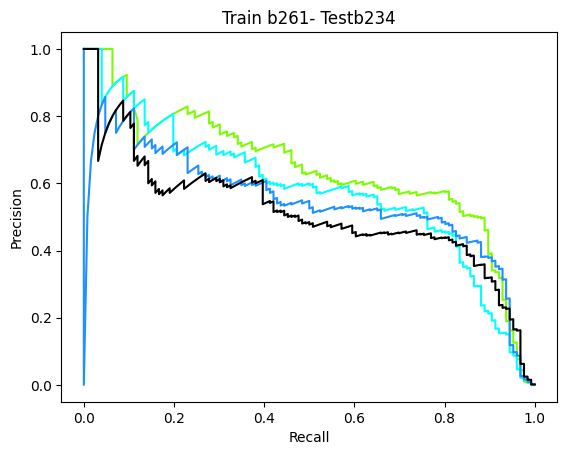
\includegraphics[width=0.25\textwidth]{Kap8/best-train=b261test=b234.png}
  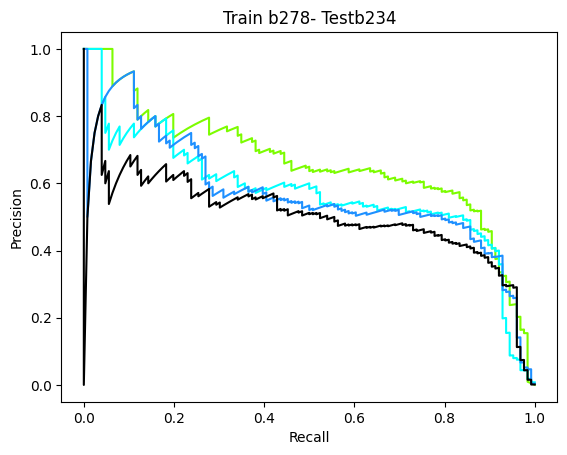
\includegraphics[width=0.25\textwidth]{Kap8/best-train=b278test=b234.png} 
   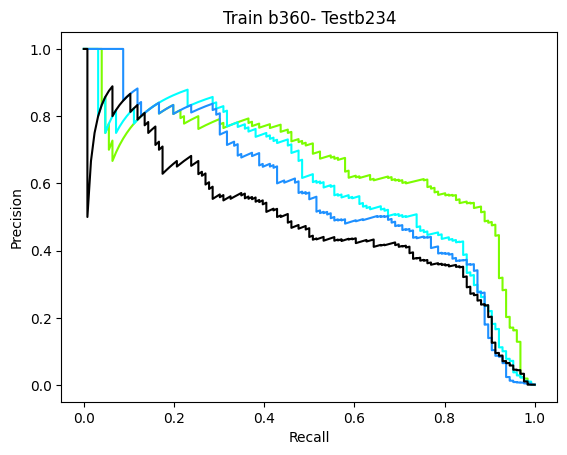
\includegraphics[width=0.25\textwidth]{Kap8/best-train=b360test=b234.png} \\

  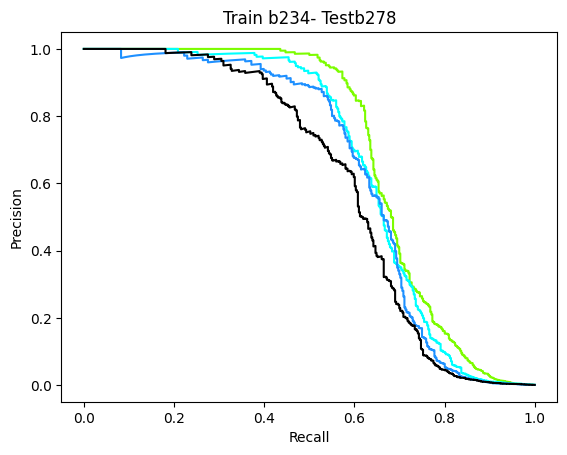
\includegraphics[width=0.25\textwidth]{Kap8/best-train=b234test=b278.png}  
  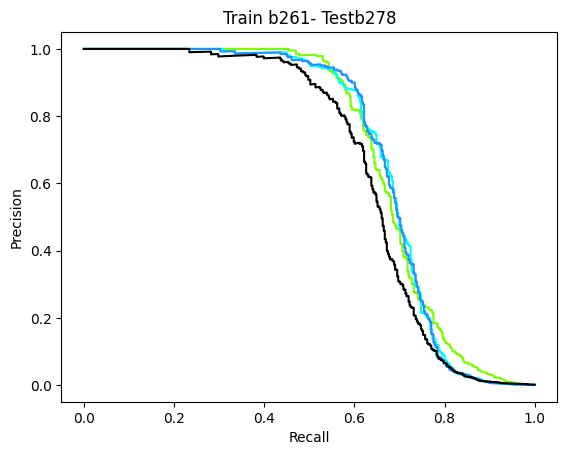
\includegraphics[width=0.25\textwidth]{Kap8/best-train=b261test=b278.png}
  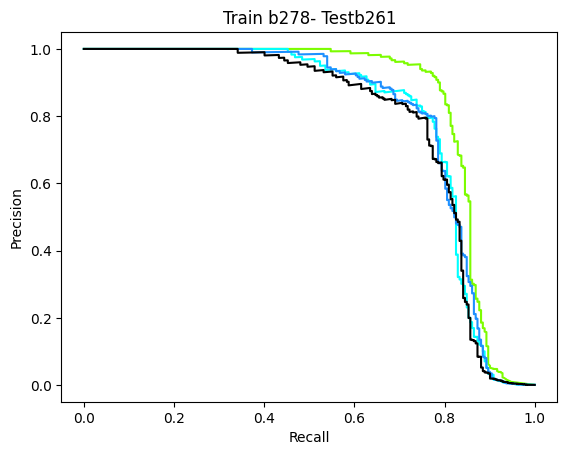
\includegraphics[width=0.25\textwidth]{Kap8/best-train=b278test=b261.png} 
   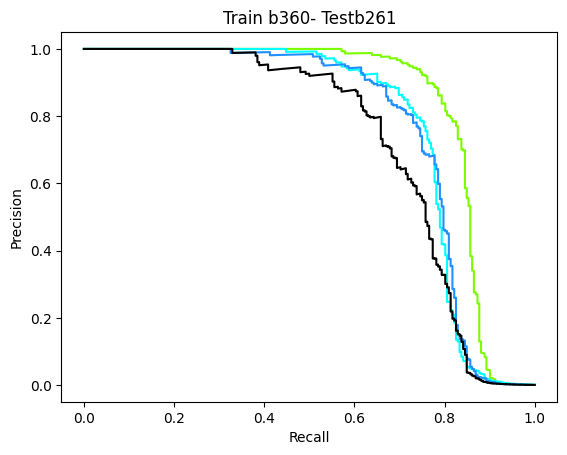
\includegraphics[width=0.25\textwidth]{Kap8/best-train=b360test=b261.png} \\
   
     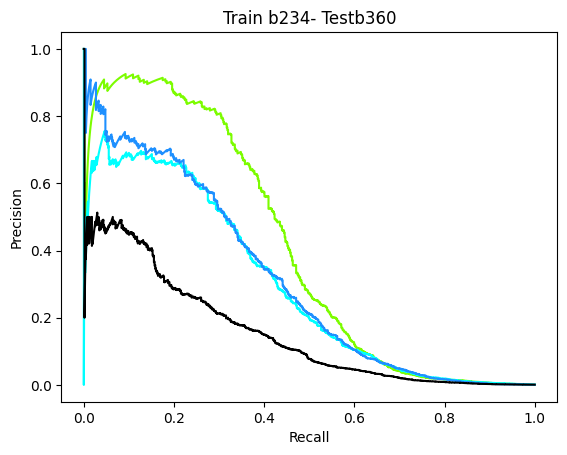
\includegraphics[width=0.25\textwidth]{Kap8/best-train=b234test=b360.png}  
  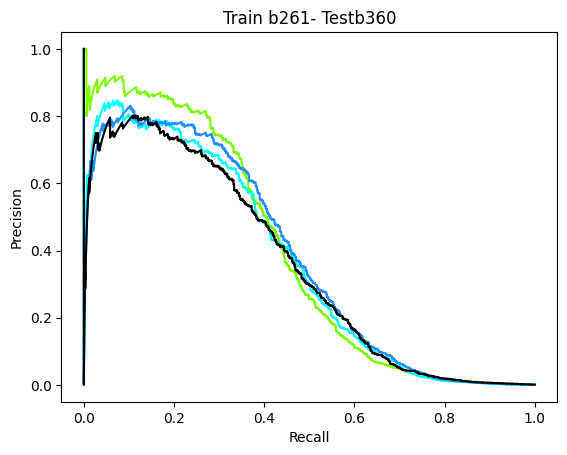
\includegraphics[width=0.25\textwidth]{Kap8/best-train=b261test=b360.png}
  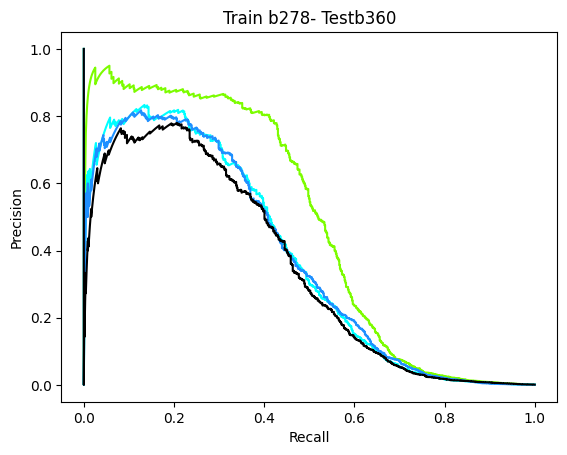
\includegraphics[width=0.25\textwidth]{Kap8/best-train=b278test=b360.png} 
   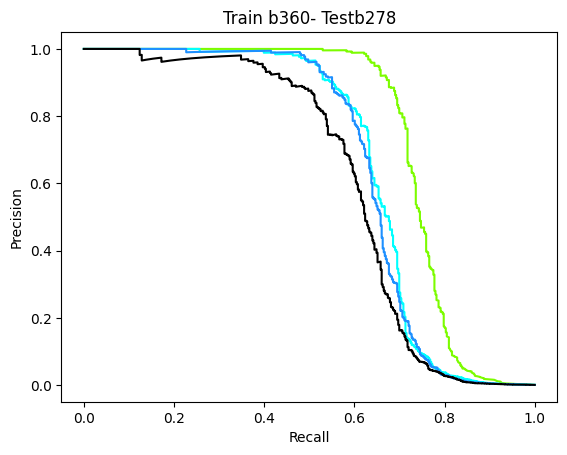
\includegraphics[width=0.25\textwidth]{Kap8/best-train=b360test=b278.png} \\

\end{tabular}
\caption{Para cada una de las grillas calculadas en la figura \protect\ref{fig:poder_predictivo}, se grafican las curvas de precision-recall correspondientes a RF y SVM-RBF con el par de parámetros óptimo de la grilla, junto con las mejores curvas de SVM-RBF y SVM-L obtenidas en capítulos anteriores. }
\label{fig:poder_predictivo_curvas}
\end{figure}

Como conclusión de este experimento, podemos descartar que la asignación de hiperparámetros escogida sea el problema por el cual SVM-RBF funciona peor que RF. Existen elecciones de hiperparámetros (como $C=10^4$ y $\gamma=10^{-4}$) que funcionan razonablemente bien en todos los pares testeados.

\section{Impacto de la variabilidad de datos en los clasificadores}

Si bien hemos comprobado que la diferencia en las distribuciones de cada tile no imposiblita hallar hiperparámetros razonables, la disparidad entre datos de entrenamiento y test puede aún estar perjudicando a SVM. En esta sección nos concentraremos en analizar esta disparidad en profundidad.

\subsection{Introducción a dataset shift}

A menudo, los científicos de datos se encuentran con que un cierto modelo funciona muy bien en los datos de entrenamiento, pero falla en obtener la misma performance en test, incluso luego de haberse asegurado de evitar sobreajustar, escogiendo el mejor modelo basado en cross-validation. En esta situación, hay algún tipo de patrón inherente a los datos de testeo que no está siendo capturado.\\

Una suposición crítica en el diseño de la amplia mayoría de algoritmos de aprendizaje automatizado supervisados es que los elementos del dataset de entrenamiento son muestreados independientemente de la misma distribución de probabilidad subyacente que los elementos sobre los cuales el modelo hará predicciones \cite{non-stationary} \cite{kouw2019introduction} \cite{selectionbias} \cite{GeetaDharani2019CovariateSA}  \cite{RePEc:hin:jnlmpe:302815}. Sin embargo, en una gran variedad de escenarios prácticos esta simple presunción suele incumplirse \cite{non-stationary} \cite{GeetaDharani2019CovariateSA} \cite{quinonero2009dataset}.  Distintos trabajos muestran que el incumplimiento de esta premisa puede afectar seriamente la performance de la mayoría de los algoritmos de clasificación clásicos, tales como SVM \cite{selectionbias}, árboles de decisión \cite{selectionbias}, regresión lineal \cite{pmlr-v51-chen16d}, y redes neuronales \cite{RePEc:hin:jnlmpe:302815}.  \\

Para ejemplificar esta problemática, consideremos una situación donde se intenta modelar el comportamiento de compra de clientes. Supongamos que los datos de entrenamiento y de testeo lucen como en la figura \ref{fig:data_shift}. El modelo será entrenado en clientes que tienen, en promedio, menor edad que los clientes con los que se testeará. Este modelo nunca habrá visto patrones de edad como los que habrá en los datos de testeo. Si la edad es un atributo importante para el problema en cuestión, la performance en test se verá afectada. \\


\begin{figure}[h!]
\centering
  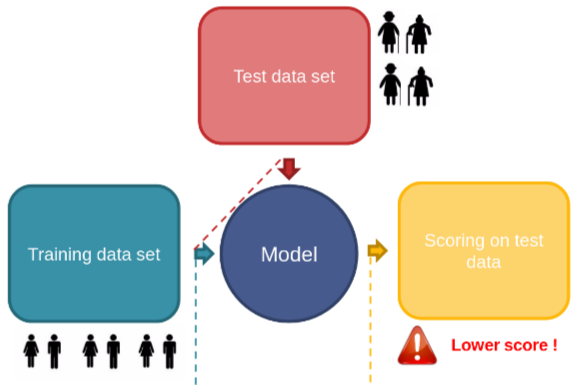
\includegraphics[width=0.6\textwidth]{Kap8/data_shift.png}  
\caption{En este ejemplo, un modelo se entrena utilizando una población joven pero se testea en una población que tiene mayor edad en promedio. Como consecuencia, el modelo no generaliza bien y se obtiene baja performance en test. Fuente: \url{analyticsvidhya.com} }
\label{fig:data_shift}
\end{figure}

Esta problemática ha recibido mucha atención en los últimos años, aunque a menudo pasa desapercibida, e incluso carece de un nombre estándar en la literatura, siendo referida con distintos nombres \cite{MORENOTORRES2012521} tales como: dataset shift \cite{quinonero2009dataset}, concept shift o concept drift \cite{widmer1998special} \cite{conceptdrift} , changing environments \cite{changingenvironments}, etc. Formalmente, definiremos \textbf{dataset shift} (variabilidad de datasets) como aquella situación en la cual la distribución de probabilidad de los datos de entrenamiento es distinta a la distribución de probabilidad de los datos de test \cite{quinonero2009dataset} \cite{non-stationary}.

\begin{center}
$ P_{train}(x,y) \neq P_{test}(x,y) $
\end{center}

La presencia de dataset shift es común en muchas aplicaciones prácticas y puede ser causada por distintos motivos, tales como:

\begin{itemize}
\item Ambientes no estacionarios: Datos obtenidos en distintas locaciones, en distintos instantes de tiempo, etcétera \cite{quinonero2009dataset} \cite{adaptative_learning} \cite{MORENOTORRES2012521}. Por ejemplo, un dataset recolectado en una cierta estación del año o en una cierta región geográfica es utilizado para realizar predicciones sobre datos recolectados en una estación del año o región geográfica notablemente distinta. 
\item Sesgo introducido por el diseño experimental mediante el cual se obtuvieron los datos \cite{MORENOTORRES2012521}. Por ejemplo, en ciencias sociales, habrá subconjuntos de una población general (e.g. estudiantes en la universidad que conduce un cierto experimento) que serán más fáciles de encuestar que otros. Tales subconjuntos de la población pueden estar sobre-representados, en tanto que otros subconjuntos (e.g. convictos) pueden ser completamente excluidos.
\item Incapacidad de reproducir las condiciones de testeo al momento de entrenar.
\end{itemize}

Algunos ejemplos de dataset shift, extraídos de \cite{quinonero2009dataset}, son:

\begin{itemize}
\item El país Albodora hizo un estudio que muestra que la introducción de una cierta medida ayudó a disminuir el consumo de alcohol en menores de edad. Los políticos de Bodalecia están impresionados y quieren reutilizar las mismas medidas. ¿Deberían?
\item Un algoritmo para detectar intrusiones en una red fue desarrollado utilizando aprendizaje automatizado en datos de hace cuatro años. ¿Funcionará hoy en día tan bien como cuando fue lanzado?
\end{itemize}

\subsection{Tipos de dataset shift}

Es interesante discriminar entre distintos tipos de dataset shift. La variedad de dataset shift más ampliamente estudiada es \textbf{covariate shift}\footnote{En este contexto, la palabra \textit{covariate} (en inglés) se utiliza como sinónimo de atributo o feature.} (también llamado covariate drift), en la cual la variabilidad entre los datos de entrenamiento y de testeo se encuentra únicamente en los atributos \cite{non-stationary} \cite{quinonero2009dataset} \cite{MORENOTORRES2012521} \cite{kouw2019introduction}. Esto se ejemplifica en la figura \ref{fig:ds_shift_sets}a. \\

Formalmente: 

\begin{center}
$ P_{train}(y|x) = P_{test}(y|x) \ \wedge \  P_{train}(x) \neq P_{test}(x)$
\end{center}

\begin{figure}[h!]
\centering
  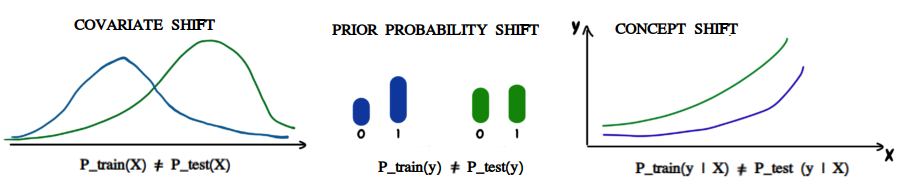
\includegraphics[width=\textwidth]{Kap8/types_of_drift.png}
\caption{ Ilustración de tres tipos distintos de dataset shift. Créditos: Pawel Cislo \url{pawelcislo.com} }
\label{fig:dataset_shift_types}
\end{figure}

Algunos ejemplos reales de covariate shift incluyen:

\begin{itemize}
\item Algoritmos de reconocimiento de rostros que son entrenados predominantemente con rostros jóvenes, pero los datos de testeo tienen una proporción mucho mayor de rostros de gente mayor.
\item Predecir la expectativa de vida pero tener muy pocas instancias en los datos de entrenamiento de individuos que fuman, y muchos más en los datos de testeo.
\item Clasificar imágenes como gatos o perros, pero omitir ciertas especies en los datos de entrenamiento que son comunes en los datos de testeo.
\end{itemize}

En particular, covariate shift puede causar muchos problemas al utilizar cross-validation. Cross-validation estimará la performance en test utilizando únicamente los datos de entrenamiento. Esta estimación no será realmente fiel a la performance en los datos de test. \cite{LOPEZ20141} \cite{10.5555/1314498.1390324} \\

Otros tipos de dataset shift se ilustran en la figura \ref{fig:dataset_shift_types} e incluyen:

\begin{itemize}
\item \textbf{Prior probability shift}: Mientras que covariate shift se concentra en cambios en los atributos $x$, prior probability shift sucede cuando únicamente  la distribución de la variable objetivo $y$ cambia \cite{quinonero2009dataset} \cite{MORENOTORRES2012521}. Esto se ejemplifica en la figura \ref{fig:ds_shift_sets}b.
\item \textbf{Concept shift}: Sucede cuando el cambio no se encuentra puntualmente en las distribuciones de probabilidad, si no que la relación entre los atributos $x$ y la variable objetivo $y$ cambia \cite{MORENOTORRES2012521} \cite{kouw2019introduction}. Concept drift puede suceder en situaciones donde los datos dependen altamente del tiempo. Por ejemplo, un modelo de aprendizaje automatizado entrenado para predecir el número de vuelos diarios en un cierto aeropuerto (ver figura \ref{fig:concept_drift}). Debido a variables que no son tenidas en cuenta por el modelo, como el contexto económico y social, la variable objetivo cambia con el tiempo. Un algoritmo entrenado con datos  de 1949 a 1950 será incapaz de realizar predicciones en acertadas sobre 1960.
\end{itemize} 

\begin{figure}[h!]
\centering
  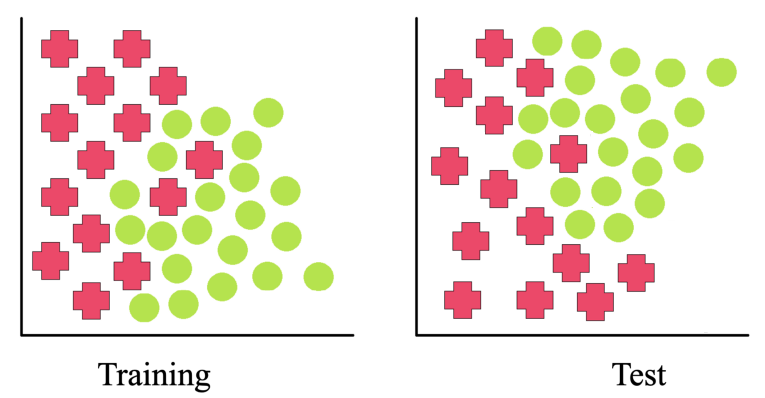
\includegraphics[width=0.6\textwidth]{Kap8/covariate_shift.png} \\
  (a) Covariate shift \\
  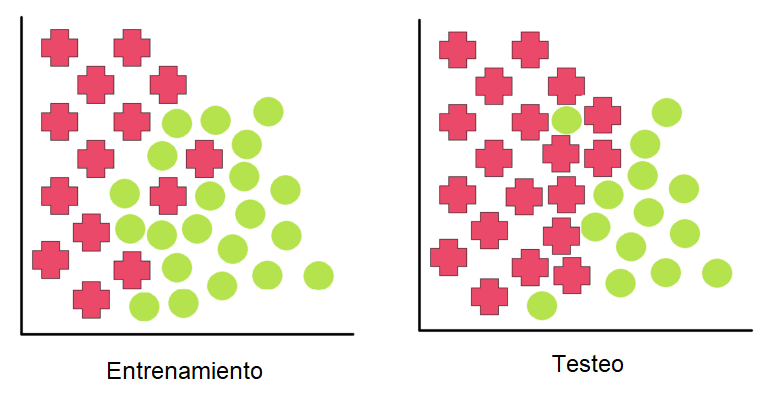
\includegraphics[width=0.6\textwidth]{Kap8/prior_shift.png}  \\
  (b) Prior shift.

\caption{Ejemplos de covariate shift (a) y prior shift (b). Notar que, en covariate shift, la probabilidad a priori de las clases no cambia entre train y test. Similarmente, en prior shift, la distribución de los atributos se mantiene constante. Créditos: \url{towardsdatascience.com}}
\label{fig:ds_shift_sets}
\end{figure}

\begin{figure}[h!]
\centering
  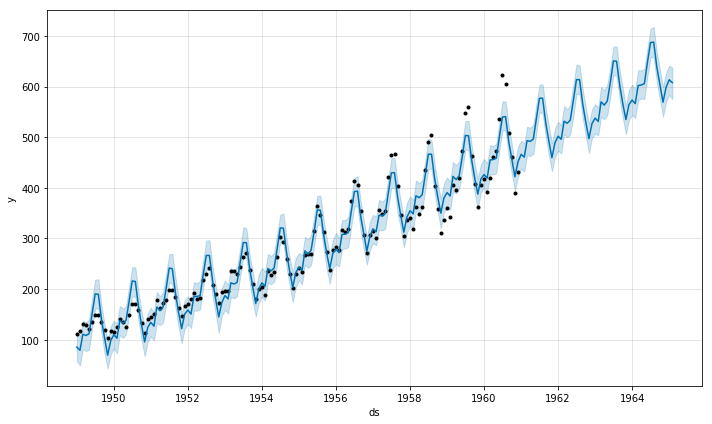
\includegraphics[width=0.6\textwidth]{Kap8/concept-drift.png}  
\caption{Cantidad de vuelos de un aeropuerto en función del tiempo. Fuente: \url{gsarantitis.wordpress.com}}
\label{fig:concept_drift}
\end{figure}

En este capítulo nos concentraremos principalmente en analizar la presencia y el impacto de covariate shift en los tiles de Carpyncho, dado que experimentos llevados a cabo en capítulos anteriores han evidenciado la presencia de esta problemática en nuestros datos (ver figura \ref{fig:distribuciones_distintas}).


\subsection{Efecto de covariate shift en SVM}

En la figura \ref{fig:svm_afectado} se ilustra el efecto perjudicial que covariate shift puede tener en SVM. En la subfigura de la izquierda, vemos el hiperplano separador óptimo que se calcula en base a los datos de entrenamiento (azul). Sin embargo, el dataset de test (rojo) exhibe una distribución de probabilidad ligeramente distinta a la distribución de entrenamiento. El hiperplano separador hallado durante la fase de entrenamiento no es capaz de separar correctamente las clases gobernadas por esta nueva distribución de probabilidad. \\


\begin{figure}[h!]
\centering
  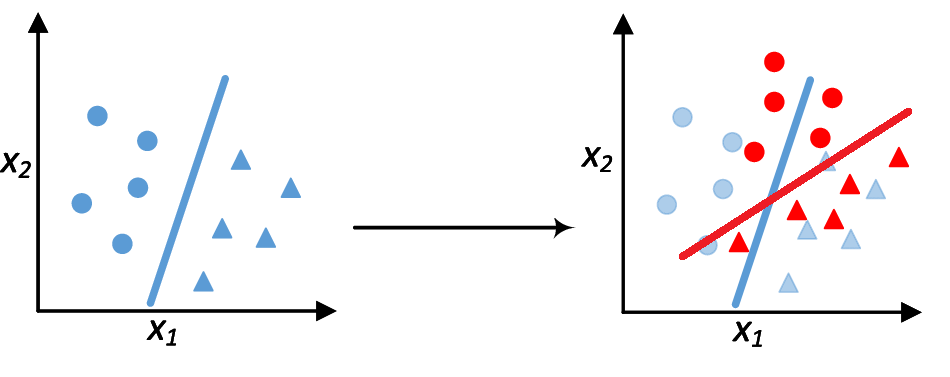
\includegraphics[width=0.6\textwidth]{Kap8/svm_afectado.png}  
\caption{En esta figura se ilustra el efecto negativo de covariate drift sobre SVM.}
\label{fig:svm_afectado}
\end{figure}

Distintos trabajos han estudiado el efecto que covariate drift tiene sobre clasificadores clásicos como  SVM como árboles de decision \cite{non-stationary}. En particular, los experimentos llevados a cabo en \cite{selectionbias} indican que los árboles de decisión toleran bastante bien la presencia de covariate drift:

\begin{quotation}
Sorpresivamente, C4.5 tiene muy buena performance en presencia de covariate drift. Esto podría ser explicado por el hecho de que, a pesar de que la elección de las divisiones en cada nodo (splits) está sesgada, las clases escogidas en las hojas no lo están.
\end{quotation}

En este mismo estudio, SVM muestra una mayor degradación en performance ante la presencia de covariate drift. Esto podría explicar por qué RF\footnote{Si bien la implementación de RF utilizada en este trabajo utiliza el algoritmo CART (ver sección \protect\ref{cart}) en vez de C4.5, ambas implementaciones son muy similares. En la sección de trabajo futuro (\protect\ref{tfuturo}) se propone extender la investigación realizada por \protect\cite{selectionbias}.} parece verse menos afectado que SVM por la presencia de covariate drift en los tiles de Carpyncho. \\

Dataset shift es especialmente perjudicial en problemas de clasificación imbalanceados, dado que la clase positiva es muy sensible a errores de clasificación individuales debido la poca densidad de ejemplos \cite{LOPEZ20141}.

\subsection{Identificando la presencia de covariate shift}

Teóricamente, a falta de mayores asunciones, cambios en la distribución de los atributos pueden causar una degradación arbitrariamente severa en la performance de clasificadores. Sin embargo, en la práctica, las distribuciones de train y test cambian constantemente, y a menudo estos cambios son benignos pues la diferencia es muy pequeña. Existe una amplia variedad de técnicas propuestas para determinar hasta qué punto los datos presentan covariate shift \cite{rabanser2019failing} \cite{GeetaDharani2019CovariateSA}, incluyendo:

\begin{itemize}
\item \textbf{Distancia estadística}: Consiste en detectar si las distribuciones son distintas utilizando métricas como PSI (Population Stability Index), Kolmogorov-Smirnov statistic, Kullback-Lebler divergence, intersección de histogramas, etcétera. Esta última es ilustrada en la figura \ref{fig:hist_intersection}. Estas técnicas, sin embargo, se vuelven más complejas de utilizar cuando los datos tienen alta dimensionalidad.
\item \textbf{Detección de novedades} (Novelty detection): Dada una nueva instancia de test, utilizar métodos de detección de novedades (o detección de anomalías) para identificar si se condice o no a la distribución de entrenamiento \cite{noveltydetection}.
\item \textbf{Distancia discriminatoria} (Discriminative distance): La intuición detrás de estos métodos es que, si hay covariate drift, entonces debería ser posible entrenar un clasificador que aprenda a separar los datos de entrenamiento y de testeo con alta performance. El error de este clasificador puede utilizarse como una medida de la distancia entre las dos distribuciones \cite{discriminative_distance} \cite{GeetaDharani2019CovariateSA}. Una ventaja de utilizar distancia discriminatoria es que puede utilizarse en dominios arbitrarios, incluyendo datos dispersos y con alta dimensionalidad.
\end{itemize}

\begin{figure}[h!]
\centering
  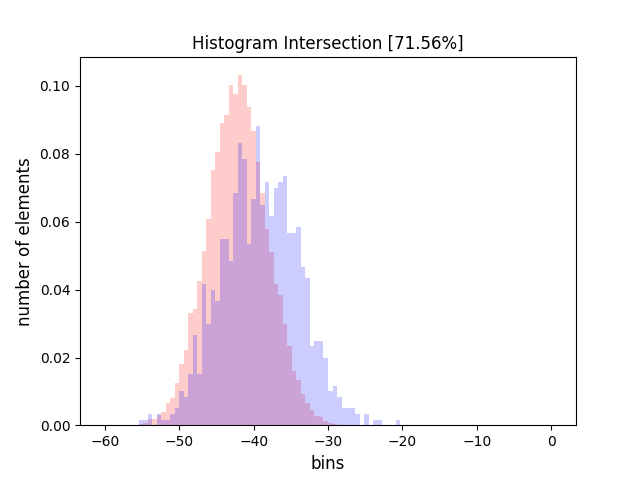
\includegraphics[width=0.6\textwidth]{Kap8/histogram_intersection.png}  
\caption{Ilustración del cálculo de la intersección de histogramas de frecuencia correspondentes a los datos de test (rosa) y training (violeta). Hay aproximadamente 72\% de intersección entre las distribuciones, lo cual indica un nivel razonable de covariate shift entre las distribuciones. Fuente: \url{towardsdatascience.com}}
\label{fig:hist_intersection}
\end{figure}

Debido a la alta dimensionalidad de los tiles de Carpyncho, se decidió utilizar distancia discriminatoria para medir el nivel de covariate drift presente. Se procedió como sigue:

\begin{enumerate}
\item Dados dos tiles $t_1$ y $t_2$, sea $n$ el mínimo entre la cantidad de filas de $t_1$ y la cantidad de filas de $t_2$. 
\item Seleccionar aleatoriamente $n$ elementos de $t_1$ y $n$ elementos de $t_2$. Descartar las viejas etiquetas a predecir (RRL o noRRL). Se combinan todos los datos en un nuevo dataset $t$. Etiquetar cada fila de $t$ con clase $1$ si proviene del $t_1$ y $0$ si proviene de $t_2$. 
\item Dividir $t$ en un conjunto de entrenamiento (75\% de los datos) y un conjunto de test (25\% de los datos).
\item Entrenar un clasificador RF y un clasificador de regresión logística (LR en adelante,\cite{statisticallearning}) utilizando el dataset de entrenamiento.
\item Utilizar ambos modelos para calcular accuracy y el área debajo de la curva ROC en test. Estas métricas son apropiadas por que $t$ es un dataset completamente balanceado.
\end{enumerate}

Algunos detalles del experimento:
f
\begin{itemize}
\item RF se utiliza con tan solo 50 árboles. Los atributos no se escalan ni se discretizan. Previamente a entrenar el clasificador, se realiza selección de 45 atributos tal y como se explicó en la sección \ref{mejores_fs}.
\item Regresión logística se realizó con C=1. Se discretizaron los atributos utilizando binning y luego se escalan utilizando un escalado estándar. Previamente a entrenar el clasificador, se realiza selección de 45 atributos tal y como se explicó en la sección \ref{mejores_fs}.
\end{itemize}

La figura \ref{fig:covariate_matrix} muestra los resultados obtenidos. En trabajos previos, se ha considerado que AUC-ROC mayor a 0.8 indica la presencia no despreciable de covariate shift \cite{GeetaDharani2019CovariateSA}. Como podemos ver, ambos clasificadores son sorprendentemente efectivos a la hora de distinguir la pertenencia a distintos tiles:

\begin{itemize}
\item Tanto LR como RF son capaces de distinguir con gran exactitud el tile de origen, LR en particular permite separar de forma casi perfecta algunos pares.
\item Vemos que el tile $b360$ presenta el mayor covariate shift al comparársele con los demás tiles, especialmente con $b234$. Esto podría explicar por qué, en la figura \ref{fig:poder_predictivo_curvas}, las curvas donde se testea con $b360$ son las peores de todo el experimento (tanto para SVM como RF). Sin embargo, resulta curioso notar que al utilizar $b360$ para entrenar, la performance es notablemente buena a pesar de que el covariate shift se mantiene constante. La variación en la distribución subyacente, aparentemente, resulta más benigna en este último caso y los modelos obtenidos generalizan bien.
\item El par $b261$ y $b278$ presenta la menor cantidad de covariate shift. Esto explicaría por qué las curvas $b261 \mapsto b278$ y $b278 \mapsto b261$ en la figura \ref{fig:poder_predictivo_curvas} son prácticamente idénticas.
\item La severidad del covariate shift detectado parece ser proporcional a la distancia espacial de los tiles (ver figura \ref{fig:vvv_tiles}). De ser cierto, sería beneficioso entrenar y testear con tiles que se encuentran espacialmente cerca, siempre que sea posible.
\item Utilizando el umbral de 0.8 AUC empleado en los trabajos previamente citados, ambos clasificadores coinciden en que todos los pares de tiles testeados se ven severamente afectados por covariate shift.
\item Nótese que se muestra la matriz completa, en vez de mostrar sólo una matriz triangular. Esto es porque se distingue entre el tile de train y entrenamiento. El tile de train define cuáles serán los 45 atributos que se mantendrán en el experimento durante el paso de selección de variables, previo a entrenar los clasificadores. A pesar de esta diferencia, vemos que el covariate shift medido con $t1 \mapsto t2$ es prácticamente el mismo que el medido con $t2 \mapsto t1$.
\item Obviamente, cuando el tile de entrenamiento y de testeo son el mismo resulta imposible distinguirlos, y los clasificadores tienen la misma performance que un clasificador aleatorio (accuracy del 50\%, área debajo de la curva ROC 0.5).
\end{itemize}

\begin{figure}[h!]
\begin{tabular}{cc}

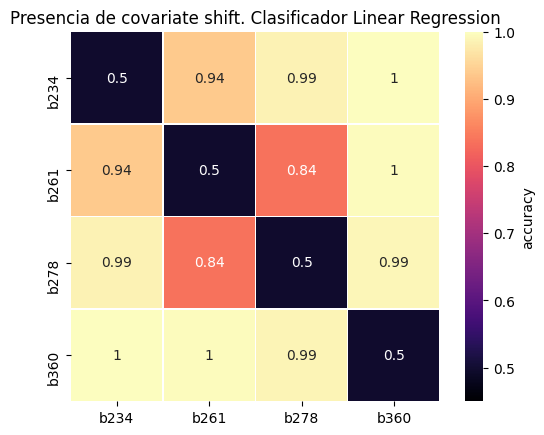
\includegraphics[width=0.49\textwidth]{Kap8/CS-Method+Linear_Regressionmetricaccuracy.png} & 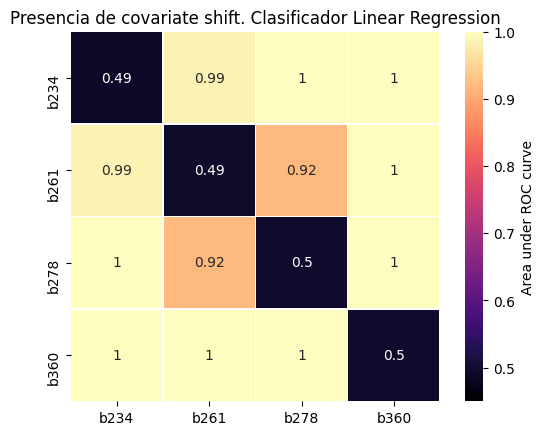
\includegraphics[width=0.49\textwidth]{Kap8/CS-Method+Linear_Regressionmetricauc.png}  \\

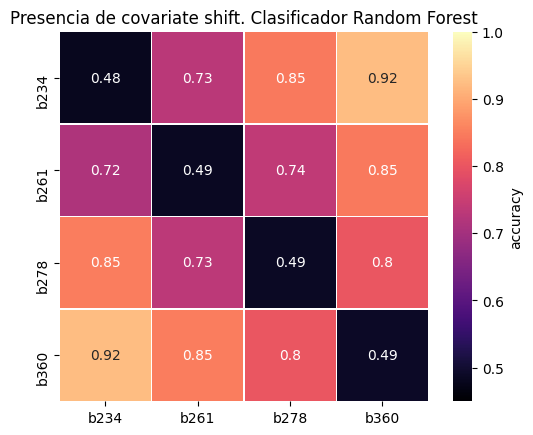
\includegraphics[width=0.49\textwidth]{Kap8/CS-Method+Random_Forestmetricaccuracy.png}  & 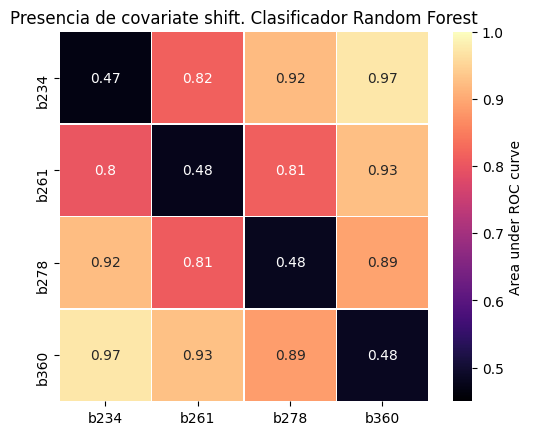
\includegraphics[width=0.49\textwidth]{Kap8/CS-Method+Random_Forestmetricauc.png} 
\end{tabular}
\caption{Cálculo de distancia discriminatoria sobre un subconjunto de tiles de la VVV. Se intenta medir el grado de separación entre las distribuciones de probabilidad de distintos tiles, entrenando clasificadores RF y LR que buscan diferenciar ambas distribuciones.}
\label{fig:covariate_matrix}
\end{figure}

\subsection{Reduciendo el impacto covariate shift}

Una vez que se ha identificado que los datos se ven afectados por covariate shift,  distintos trabajos han propuesto multitud de técnicas para mitigar el efecto que tiene en performance. Algunas de las ideas más predominantes son:

\begin{itemize}
\item \textbf{Importance reweighting}: Consiste en aumentar la importancia de aquellos elementos del conjunto de entrenamiento que son más similares a las instancias en test  \cite{kouw2019introduction} \cite{non-stationary}  \cite{GeetaDharani2019CovariateSA}. Esencialmente, se intenta sesgar al clasificador para que preste más atención a aquellos datos de entrenamiento que se parecen más a los datos de test. Esto se ilustra en la figura \ref{fig:histogram_intersection}.

\item \textbf{Eliminar atributos que causan covariate shift}: Eliminar aquellos atributos que más contribuyen a la diferencia entre datasets. Una forma de hacer esto es, nuevamente, utilizando la idea de distancia discriminatoria desarrollada en la sección anterior:

\begin{itemize}
\item Luego de entrenar un clasificador que distinga entre los datos de entrenamiento y de test, puede estimarse qué atributos son más importantes para el modelo (utilizando importancia gini en RF, por ejemplo). Aquellos atributos que no son fundamentales para el problema de clasificación original, y que contribuyen notablemente a diferenciar el tile de train del de test, pueden ser eliminados. Esto se ilustra en la figura \ref{fig:discriminative_removal}. 
\item Una segunda opción es, para cada atributo, entrenar un clasificador que utilice únicamente ese atributo para distinguir entre puntos de test y train. Aquellos atributos cuyo clasificador alcance un ROC-AUC en test mayor a un cierto umbral, por ejemplo 0.8 (\cite{GeetaDharani2019CovariateSA}), son candidatos a ser eliminados.
\end{itemize}
\end{itemize}

Variaciones de los métodos recién explicados pueden consultarse en \cite{adaptative} \cite{liu2017robust} \cite{10.5555/1314498.1390324}  \cite{adaptative_learning} \cite{kouw2019introduction}. La mayoría de los trabajos muestran claramente que hay algún beneficio en \textit{hacer algo diferente} ante la presencia de covariate shift. Sin embargo, esto debe ser evaluado con cuidado pues la mayoría de los métodos requiere el uso de los datos de testing, si bien no etiquetados, durante la fase de entrenamiento. Esto puede considerarse filtrado de información, o ser simplemente imposible. \\

\begin{figure}[h!]
\centering
  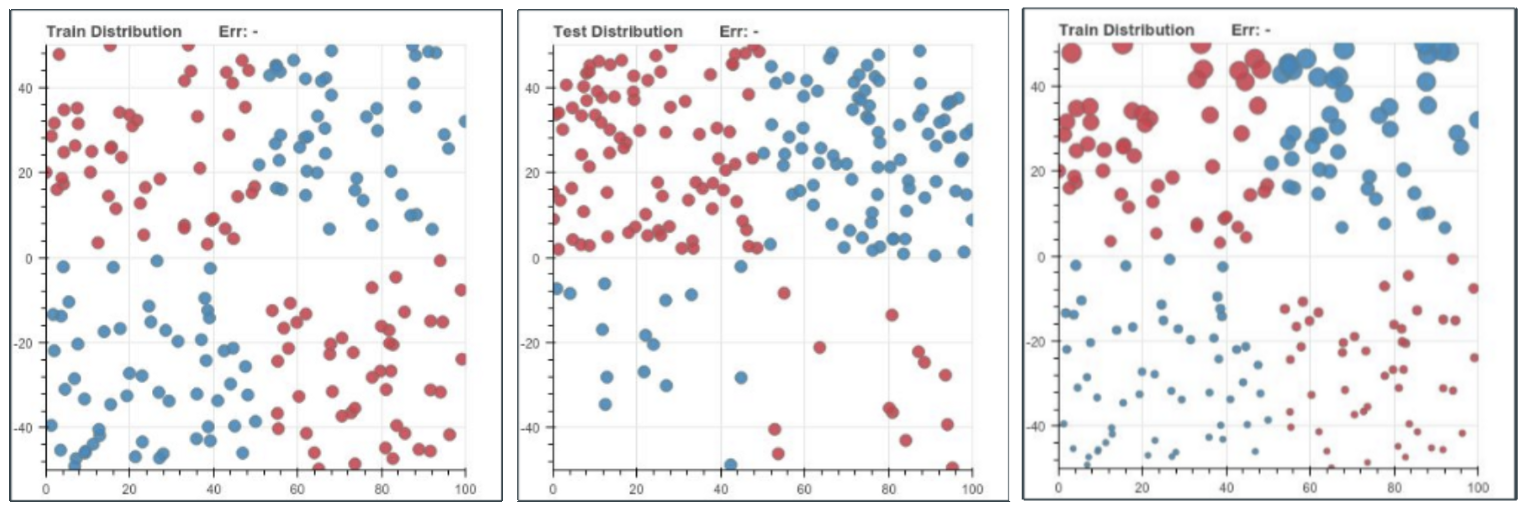
\includegraphics[width=\textwidth]{Kap8/reweighting.png}  
\caption{Importance reweighting consiste en modificar el peso de cada instancia de entrenamiento, en base a la probabilidad relativa de los datos de entrenamiento y los datos de testeo. Fuente: \url{towardsdatascience.com}}
\label{fig:histogram_intersection}
\end{figure}

\begin{figure}[h!]
\centering
  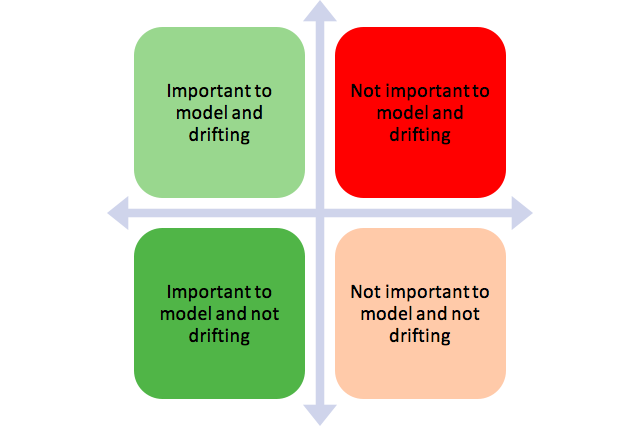
\includegraphics[width=0.6\textwidth]{Kap8/discriminative_removal.png}  
\caption{Ante la presencia de covariate drift en un problema de clasificación, podemos clasificar los atributos en cuatro grupos. Por un lado cada atributo contribuye en cierto grado a la presencia de covariate drift, y por otro lado cada atributo tiene una cierta importancia para el problema de clasificación original. Se prefiere eliminar aquellos atributos que contribuyen en mayor medida a la presencia de covariate drift, y que no son vitales para modelar el problema original. Fuente: \url{kdnuggets.com}}
\label{fig:discriminative_removal}
\end{figure}

Es factible aplicar los dos métodos recién descriptos a nuestro problema de clasificación de RRLs. En primer lugar, tanto RF como SVM permiten asignar un cierto peso o importancia a cada elemento de los datos de entrenamiento, lo cual posibilita el uso de importance reweighting. Hay una amplia variedad de técnicas propuestas para calcular los pesos adecuados, pero se ha decidido no aplicarlas en este trabajo para mantener la longitud del mismo acotada. Sería, sin embargo, muy interesante explorar los potenciales beneficios que se podría obtener. \\

Se optó por intentar eliminar atributos que causan covariate shift, estudiando puntualmente el par de tiles $b360-b234$, pues muestra la mayor divergencia. En primer lugar, se analizó la importancia de cada variable a la hora de diferenciar entre $b360$ y $b234$. Esta importancia se obtiene a partir de los clasificadores entrenados en la sección anterior; en el caso de RF es la importancia gini y en el caso de LR se obtienede forma transparente a partir de los coeficientes asignados a cada variable \cite{molnar2019}. \\

En la figura \ref{fig:covariate_ranking} se muestra, para cada atributo, la importancia obtenida por RF y LR (normalizada) a la hora de separar ambos tiles. Notar que se aplicó selección de variables previamente, por lo tanto sólo 45 atributos fueron evaluados. Los atributos están ordenados en el eje $x$ de acuerdo a su importancia para clasificar RRLs en el tile b360, de acuerdo a mutual information (ver sección \ref{experimentos_test_estadisticos}). Algunas observaciones:

\begin{itemize}
\item Tanto RF como LR señalan mayormente a atributos de color entre los más informativos para distinguir entre b360 y b234. Es decir, los atributos de color contribuyen mucho a la presencia de covariate shift. Quizás sea necesario realizar algún tipo de preprocesamiento extra de tal forma que los datos de color sean más homogéneos entre distintos tiles.
\item Los 6 atributos más importantes para distinguir RRLs y no-RRLs (de acuerdo a mutual information) parecen no contribuir significativamente a la presencia de covariate drift.
\end{itemize}

\begin{figure}[h!]
\centering
  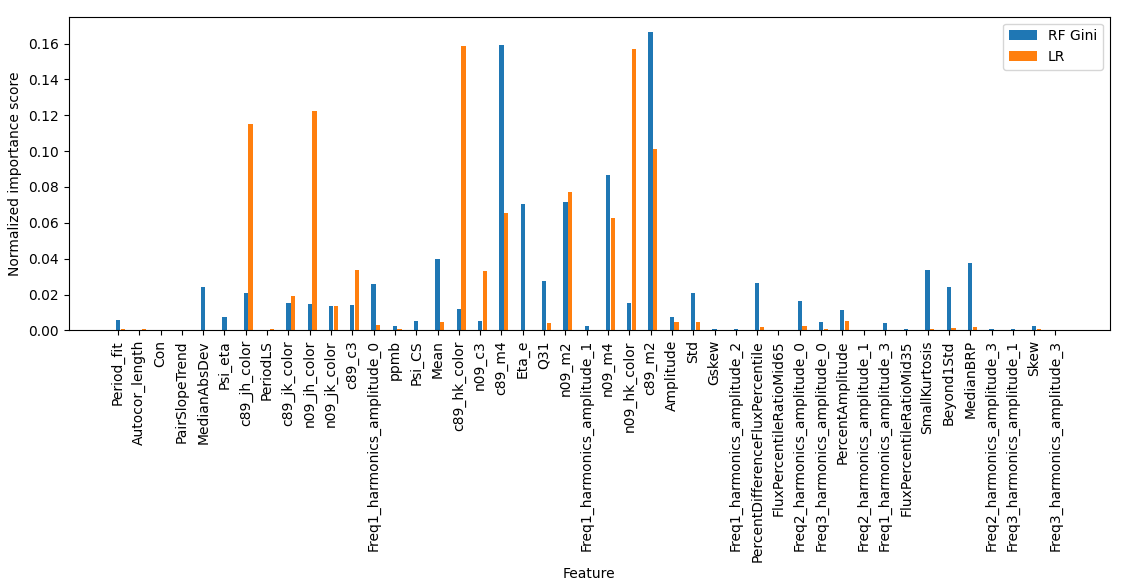
\includegraphics[width=\textwidth]{Kap8/shift_scores.png}  
\caption{Importancia de cada atributo a la hora de distinguir entre elementos de b360 y b234 provista por clasificadores RF y LR. Los puntajes de importancia provistos por cada método se muestran normalizados (de tal forma que la suma de todos los puntajes sea 1), pero no son directamente comparables entre distintos métodos.}
\label{fig:covariate_ranking}
\end{figure}

Habiéndose obtenido los puntajes de importancia para cada atributo, se procedió a evaluar cuánto disminuye la presencia de covariate drift al eliminar (uno a uno) los atributos que más contribuyen. Sin embargo, se omite eliminar aquellos atributos que se encuentran entre los 5 atributos que más contribuyen a diferenciar RRL de no-RRL de acuerdo a mutual information, para evitar perder información crítica. Los resultados se presentan en la figura \ref{fig:reduction_cd}. Algunas observaciones:

\begin{figure}[h!]
\centering
  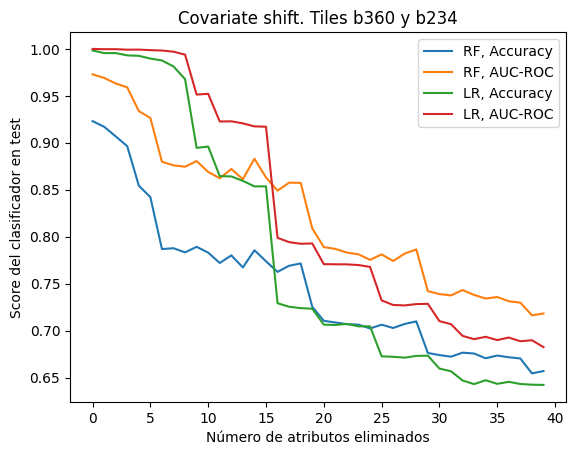
\includegraphics[width=0.6\textwidth]{Kap8/CS-Reduction-tile1b360tile2b234_single=False.png}  
\caption{En esta figura se muestra cómo se degrada la capacidad de RF y LR de distinguir entre b234 y b360 al eliminar atributos que contribuyen notoriamente a la presencia de covariate drift.}
\label{fig:reduction_cd}
\end{figure}

\begin{itemize}
\item Podemos ver que la capacidad de distinguir entre b360 y b234 efectivamente se degrada al eliminar atributos que causan covariate drift. En particular, RF pierde performance mucho más rápido; en tanto que LR recién comienza a perder performance a partir de 10 atributos eliminados.
\item Si deseamos disminuir la distancia discriminatoria a menos de 0.8 AUC, se necesita eliminar aproximadamente 20 atributos. Esto tiene un costo asociado, pues la pérdida de información puede degradar la performance en el problema de clasificación original.
\end{itemize}

El hecho de que la presencia de covariate drift no disminuya lo suficientemente rápido al eliminar los primeros atributos puede deberse a los siguientes motivos:

\begin{itemize}
\item El drift podría estar distribuido entre todos los atributos, por lo que los clasificadores pueden utilizar los atributos aún no eliminados para dividir entre b234 y b360 con alta efectividad.
\item Algún atributo que tiene alta capacidad de diferenciar entre b234 y b360 no fue eliminado por que mutual information lo considera importante para separar RRL y no-RRL.
\end{itemize}

Para poder aclarar esta situación, se procedió a entrenar un clasificador por cada atributo. La tarea del clasificador nuevamente será intentar distinguir entre elementos de b234 y elementos de b360, pero esta vez utilizando únicamente un atributo. Los resultados se encuentran en la figura \ref{fig:covariate_ranking_single}, y nos permiten apreciar que casi todos los atributos contribuyen a la presencia de covariate drift. Esto se deduce del hecho de que prácticamente todos los clasificadores individuales tienen mejor performance que un clasificador aleatorio. En particular, los atributos de color muestran nuevamente ser los más informativos para separar tiles.  \\

\begin{figure}[h!]
\centering
  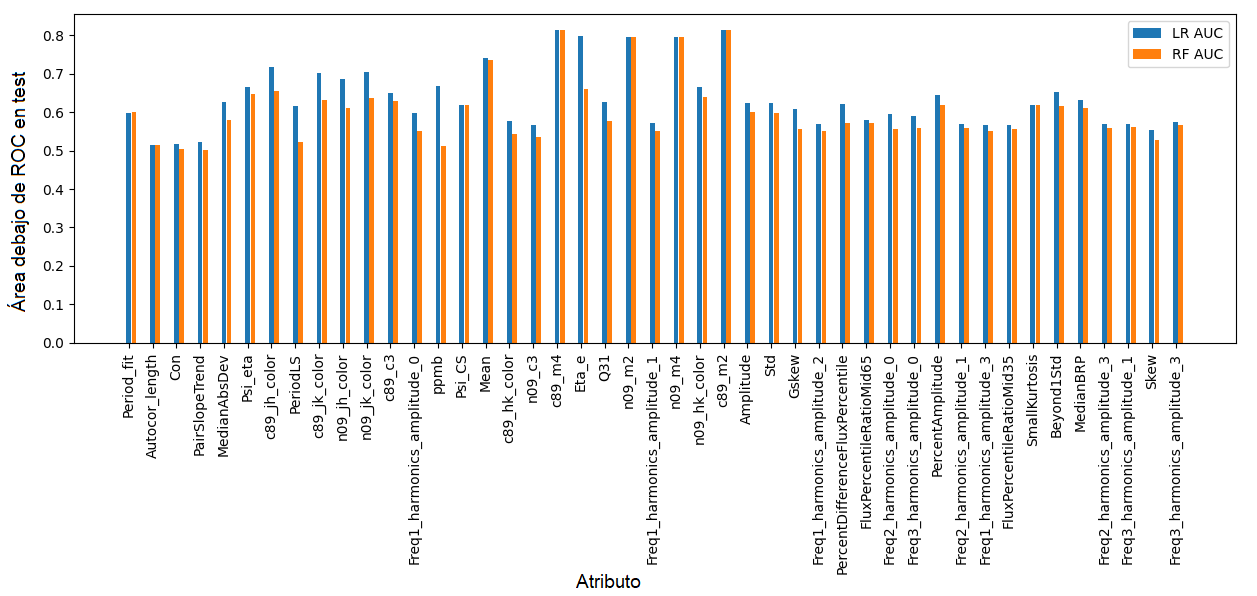
\includegraphics[width=\textwidth]{Kap8/shift_scores_single.png}
\caption{Estas figuras muestran la capacidad de cada atributo a la hora de distinguir entre b360 y b234. Por cada atributo, se entrenó un clasificador que utiliza únicamente ese atributo para distinguir entre b234 y b360. }
\label{fig:covariate_ranking_single}
\end{figure}

Finalmente, una vez identificados los atributos que más contribuyen a la presencia de covariate drift, se procedió a evaluar si eliminarlos conduce a algún beneficio en el problema de clasificación original. Para ello, se entrenó SVM-RBF en b360, testeando en b234 utilizando los preprocesamientos e hiperparámetros óptimos hallados en la sección \ref{mejores_fs}. Antes de entrenar el clasificador, se eliminan los $n$ atributos que más contribuyen a la presencia de covariate drift, omitiendo eliminar aquellos que se encuentran entre los 5 más importantes para distinguir RRLs de noRRLs.  \\

Desafortunadamente, no se observó mejoría alguna en R-AUPRC. Esto puede deberse a que es necesario eliminar demasiados atributos para reducir el covariate drift significativamente, y la pérdida de información asociada es demasiado grande. 


\section{Conclusiones}

En este capítulo se verificó, utilizando distancia discriminatoria, que el problema de clasificación que se aborda en esta tesina sufre de un fenómeno denominado covariate shift, en el cual las distribuciones de probabilidad de los datos de entrenamiento y de testeo son significativamente distintas. \\

Si bien en la sección \ref{impacto} se verificó que esto no imposibilita hallar hiperparámetros adecuados para todos los tiles, la presencia de covariate drift se propone como una explicación razonable a la disparidad de performance en clasificación que se ve al utilizar distintos tiles de entrenamiento y testeo. \\

Se intentó reducir el impacto de covariate shift eliminando los atributos que más contribuyen a distinguir distintos tiles. Sin embargo, esta técnica no logró mejorar la performance de los clasificadores SVM. Es probable esto se deba a que prácticamente todos los atributos contribuyen a la disparidad entre distintos tiles, y eliminar tan solo un puñado de atributos no logrará corregir la disparidad global de los distintos tiles. Se propone el uso de técnicas más sofisticadas, como importance reweighting, como alternativas interesantes para explorar en trabajos futuros. \\

Trabajos previos indican que los árboles de decisión se ven menos afectados por covariate shift que SVM. Esto se condice con el hecho de que todos los pares de tiles donde RF supera en performance a SVM estén entre aquellos que maximizan la presencia de covariate shift.